\chapter{Introduction}

\section{Background}

We are constantly exposed to foreign antigens; they are present on the surface of microbes and viruses or as stand-alone molecules such as toxins. Our immune system uses a variety of mechanisms to protect us. Two important mechanisms are innate and adaptive immunity. Innate immunity acts as a first line of defence and includes physical and chemical barriers; as well as other immune action from complement and non-specific responses. Adaptive immunity utilises large y-shaped proteins known as antibodies to target specific molecules named antigens. Each arm of the antibody houses a binding region \cite{edelmanAntibodyStructureMolecular1973} named a paratope responsible for binding its complementary antigen on its epitope, a singular antigen can have multiple epitopes (\textbf{Figure \ref{fig:AntibodyStructure}}). The specificity of antibodies allows them to carry out several important functions to neutralise pathogens. For example, binding to virus surface proteins can block fusion events, preventing cell infection \cite{chenHumanMonoclonalAntibodies2020}. Furthermore, antigens can aid in innate immunity by binding to phagocytes via the F\textsubscript{C} regions, inducing phagocytosis to neutralise pathogens faster \cite{forthalFunctionsAntibodies2014b}. The antibody paratopes are incredibly specific, due to their high binding affinity for their epitope counterparts and low binding affinity for other molecules, this specificity makes them useful for therapeutic and diagnostic applications.

\begin{figure}
    \centering
    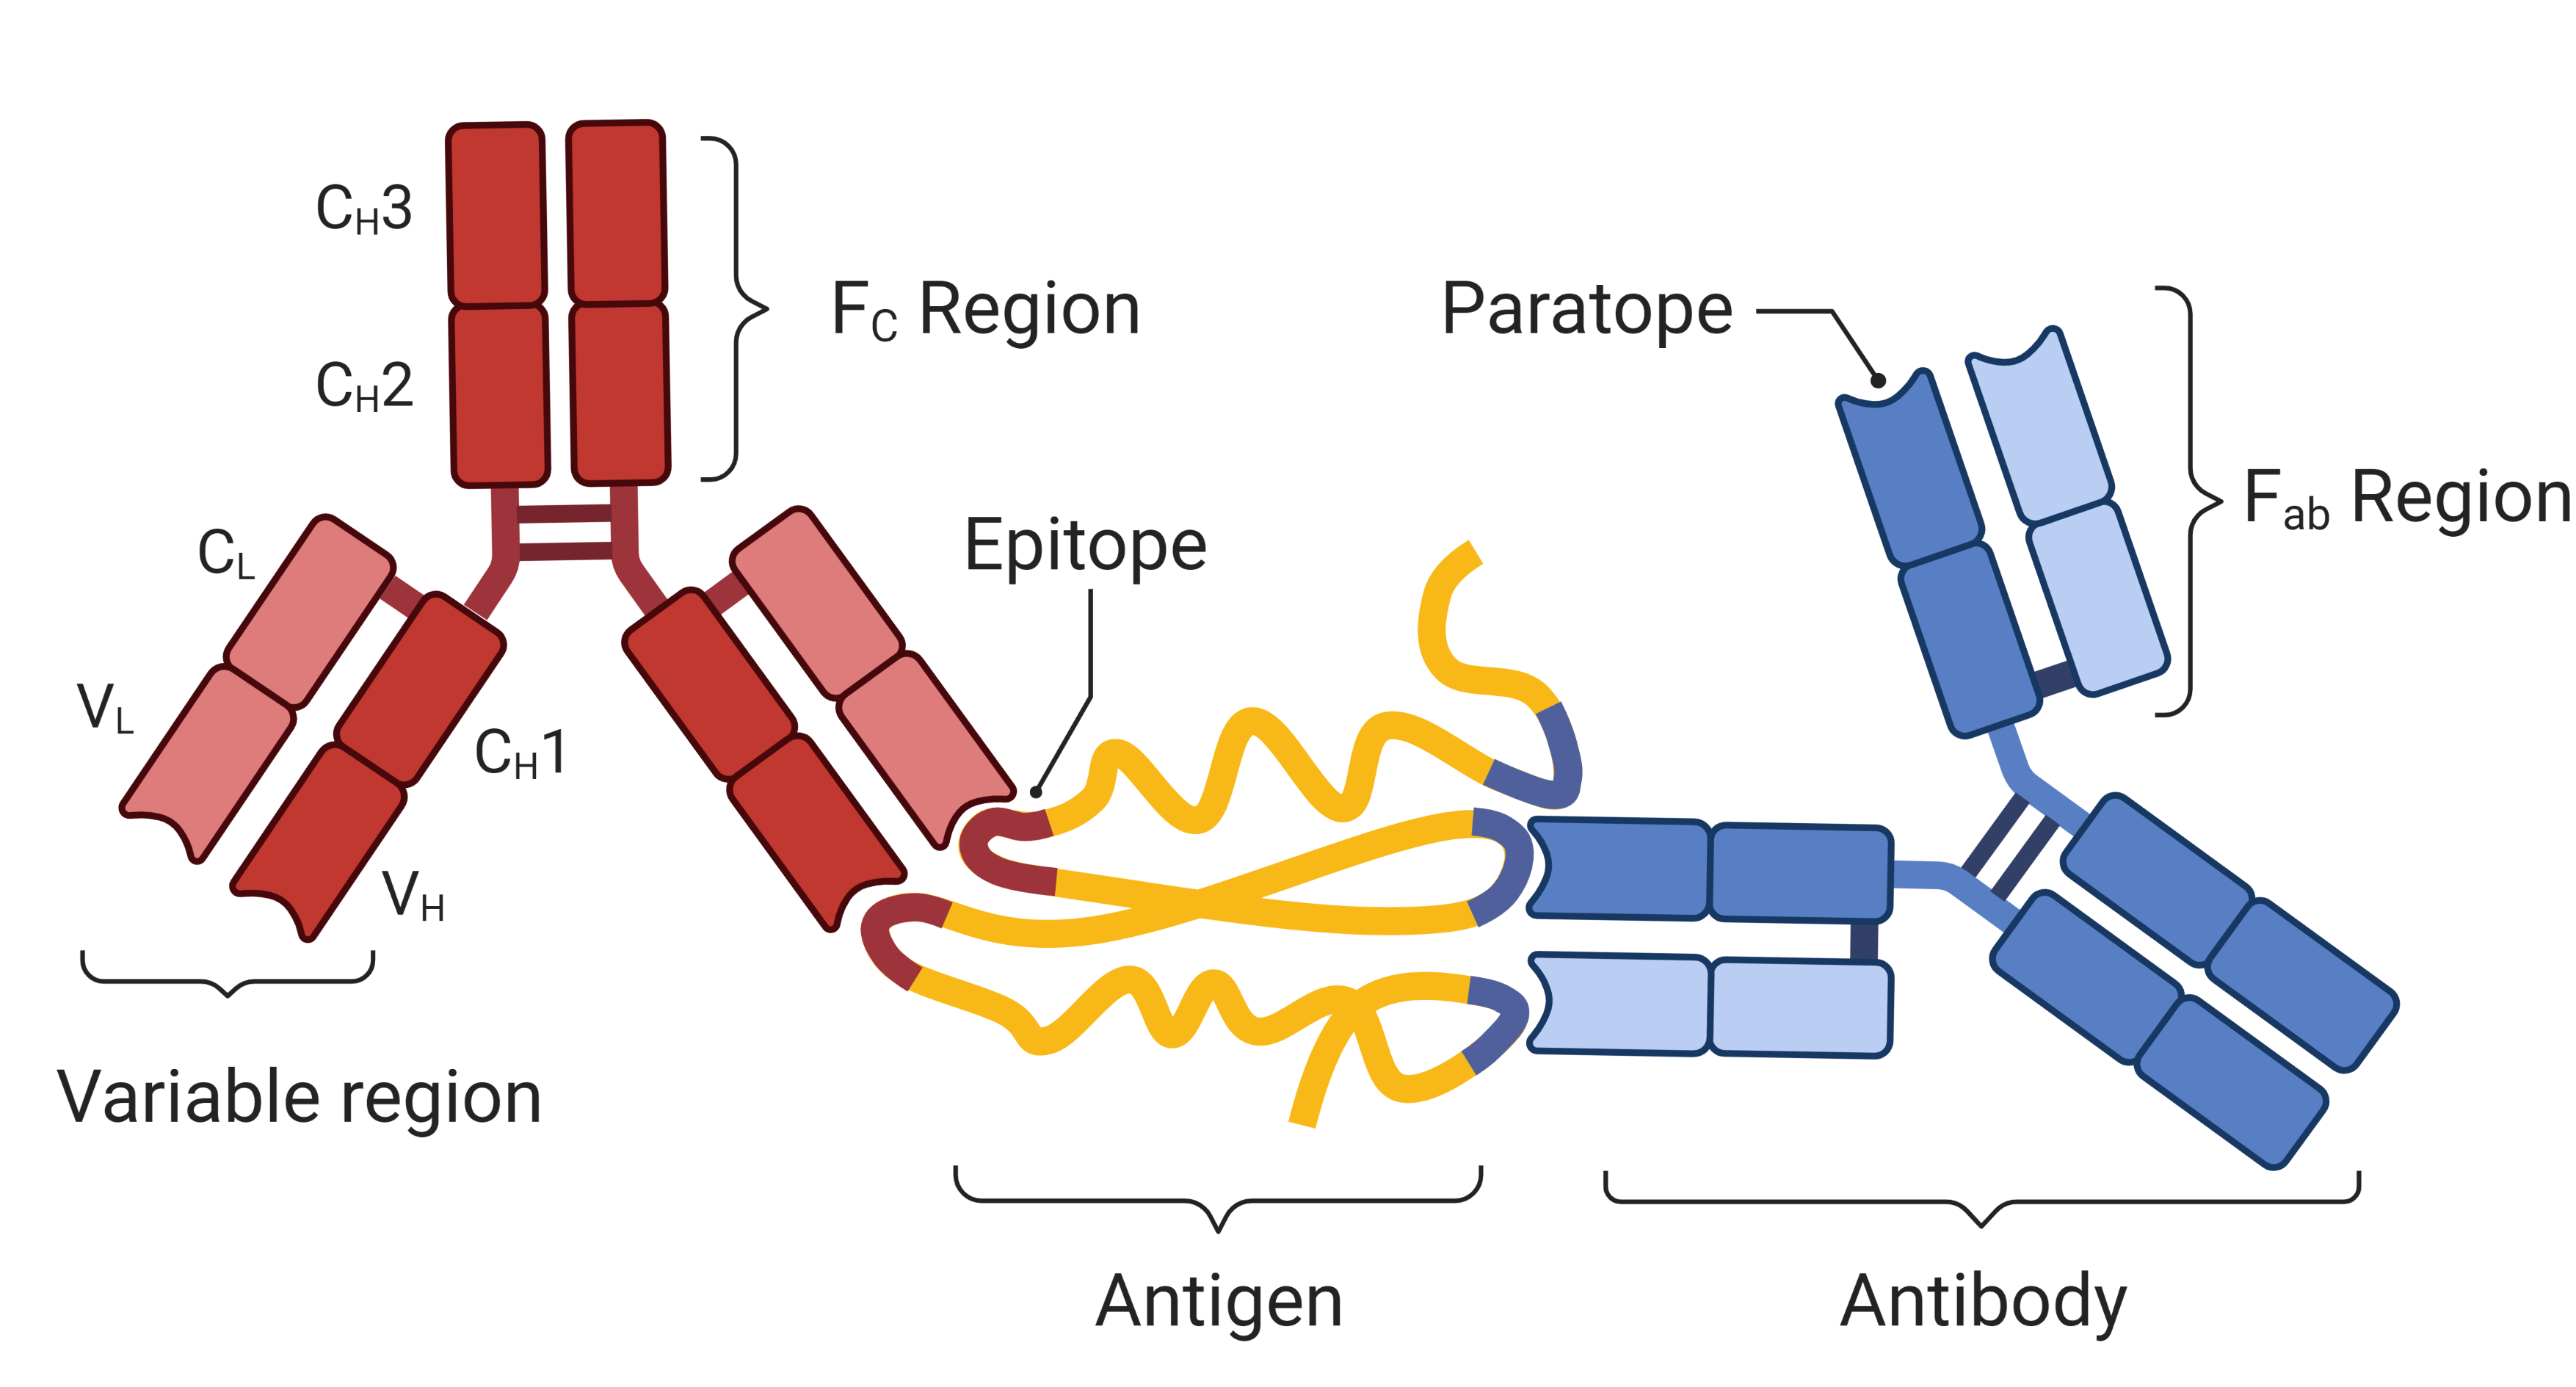
\includegraphics[width=0.9\linewidth]{./images/antibodies.png}
    \caption{\textbf{Immunoglobulin G structure} Author adapted from “Antigen Recognition by Antibodies Description”, by BioRender.com. IgG is formed from four chains; Sections C\textsubscript{H}3, C\textsubscript{H}2, C\textsubscript{H}1, and V\textsubscript{H} make up the heavy chains of ~50 kDa each and C\textsubscript{L} and V\textsubscript{L} make up the light chains of ~25 kDa each \cite{edelmanAntibodyStructureMolecular1973}.}
    \label{fig:AntibodyStructure}
\end{figure}

\subsection{Monoclonal antibodies and their production}

\begin{figure}
    \centering
    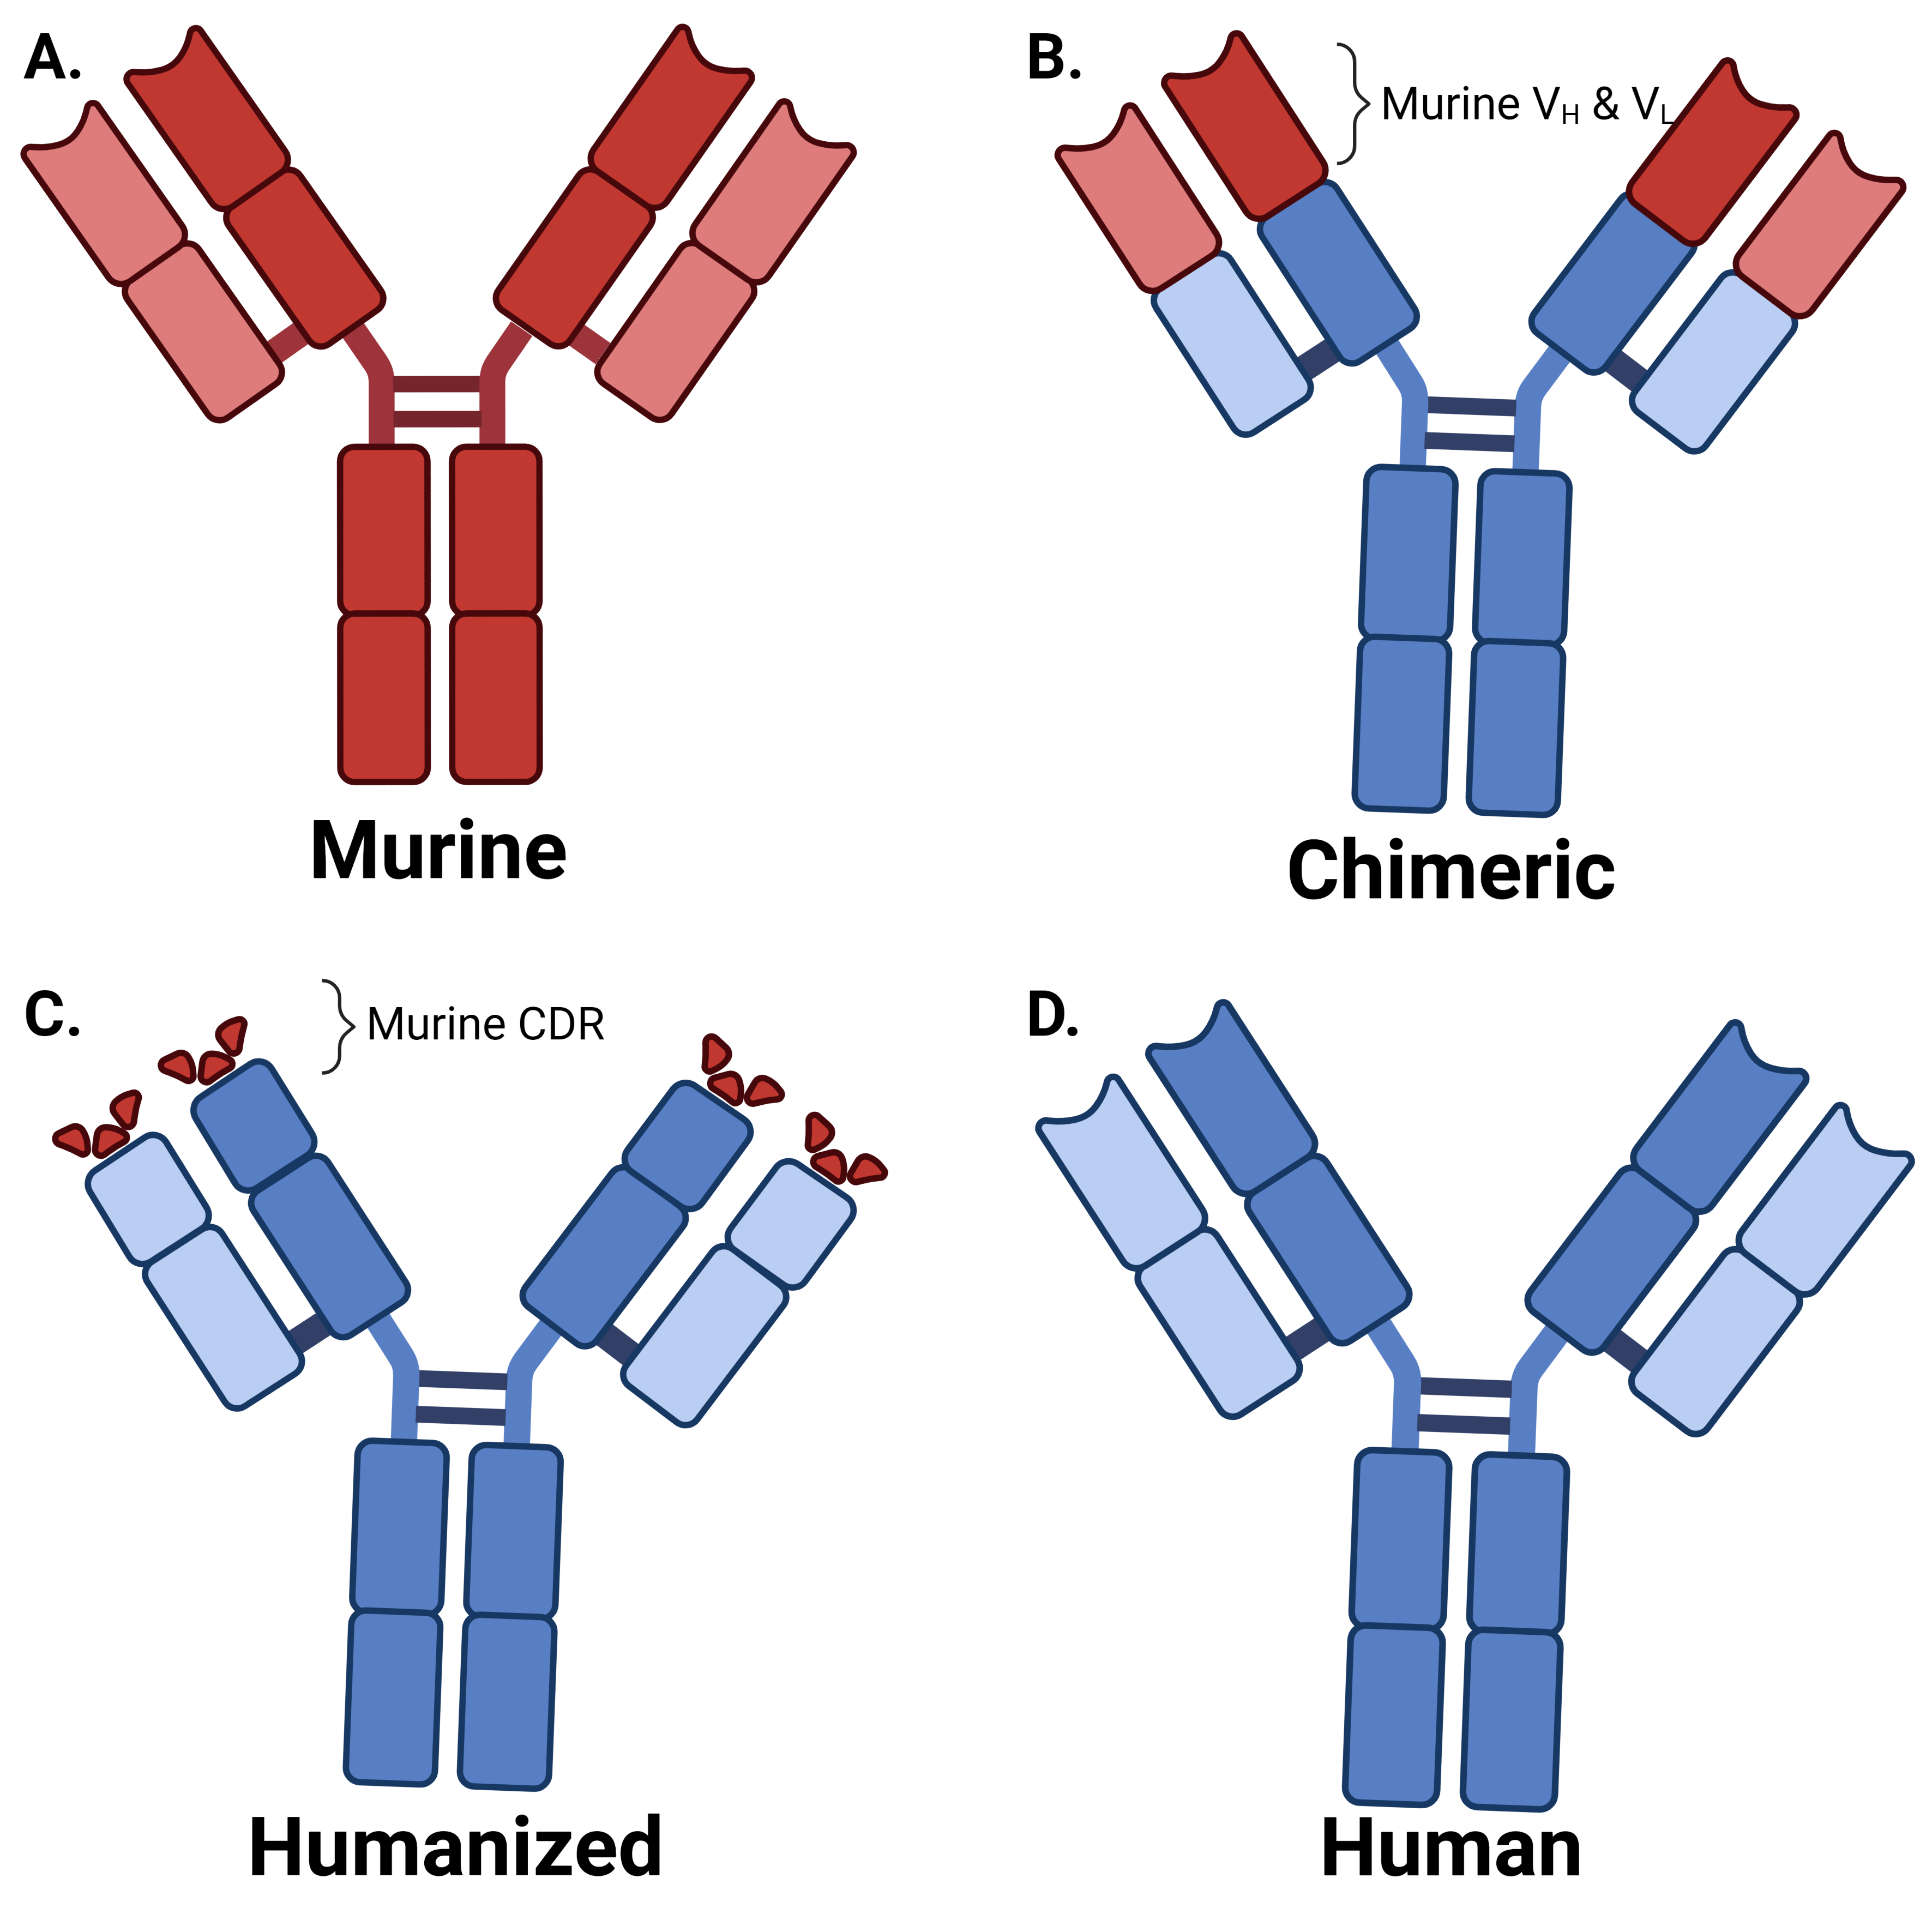
\includegraphics[width=0.6\linewidth]{./images/mabstype.png}
    \caption{\textbf{Four types of monoclonal antibody. Created with biorender.com} Murine domains are shown in red and human domains in blue. This shows the variation between a full murine mAb (a), a chimeric mAb (b) containing the variable regions from a murine antibody, a humanised mAb (c) that is mostly human domains apart from the hypervariable regions, a fully human mAb (d).}
    \label{fig:mabstype}
\end{figure}
Monoclonal antibodies (mAbs) are antibodies generated from clones of a single B lymphocyte and therefore possess identical paratopes. Their use in therapeutics is becoming increasingly popular due to their ability to bind to a large range of targets, this is reflected in the doubling of their market value between 2012 and 2017 \cite{griloIncreasinglyHumanProfitable2019}. Four key types of mAbs are: murine, chimeric, humanised, and human (\textbf{Figure \ref{fig:mabstype}}). The first therapeutic mAb was of murine descent and was released in 1986 \cite{eckerTherapeuticMonoclonalAntibody2014} under the name Orthoclone. It aimed to solve transplant rejection by targeting the CD\textsubscript{3} protein on T-cells. Murine mAbs are produced via cells known as hybridomas, a concept which was developed in 1975 by C. Milstein, G. J. F. K\"{o}hler, and N. K. Jerne for which they later received a Nobel Prize \cite{kohlerContinuousCulturesFused1975}. They injected their antigens (sheep red blood cells) into a mouse, allowing the B lymphocytes to mature and differentiate into antibody-producing plasma cells via CD4\textsuperscript{+} T lymphocyte activation \cite{breitfeldFollicularHelperCells2000}. These B lymphocytes were then extracted from the spleen of the mouse and fused with murine myeloma cells lacking the hypoxanthine-guanine phosphoribosyltransferase (HGPRT) gene, to form hybridomas. To ensure the survival of HGPRT+ fused hybridomas, they were grown on a hypoxanthine-aminopterin-thymide (HAT) medium. Aminopterin inhibits dihydrofolate reductase \cite{stoneInhibitionDihydrofolateReductase1984}, a vital enzyme in the \emph{de novo} synthesis pathway. HGPRT catalyses the formation of purine nucleotides from guanine or hypoxanthine in a process known as the salvage pathway. Therefore, unfused myelomas in the HAT medium will not replicate as neither the salvage pathway nor \emph{de novo} pathway can synthesise DNA. However, fused hybridomas have functional HGPRT translated from the B-cell genome can produce DNA via the salvage pathway and replicate. Once hybridomas have proliferated in the HAT medium their antibody products are tested using an enzyme-linked immunosorbent assay (ELISA) which confirms binding affinity for the antigen, the hybridoma with the highest affinity is selected and antibody proteins are extracted.
\\[24pt]
Unfortunately, murine mAbs do not act as effective therapeutics. On ingestion, the immune system targets these murine mAbs with human anti-murine antibodies (HAMAs), especially on repeated exposure. This leads to undesirable side effects such as an increased speed of clearance and possibly an allergic reaction \cite{hosonoHumanMouseChimeric1992,legouffeHumanAntimouseAntibody1994}. Chimeric mAbs use a human constant region (C\textsubscript{H}3, C\textsubscript{H}2,  C\textsubscript{H}1, C\textsubscript{L} (\textbf{Figure \ref{fig:AntibodyStructure}})) with murine variable regions. This proved effective, resulting in a large immunogenicity reduction \cite{hwangImmunogenicityEngineeredAntibodies2005}, suggesting HAMA antibodies mainly targeted one of the F\textsubscript{C}, C\textsubscript{L}, or C\textsubscript{H}1 regions on the murine mAbs \cite{hosonoHumanMouseChimeric1992}. The next-generation humanised mAb (\textbf{Figure \ref{fig:mabstype}.C}) only included the murine hypervariable complementary determining regions (CDRs) \cite{hardingImmunogenicityHumanizedFully2010}. CDRs are responsible for forming the paratope and are the loops that contact the antigen. This further reduces the HAMA response, but to minimise immune action a requirement for human antibodies arose.
\begin{figure}
    \centering
    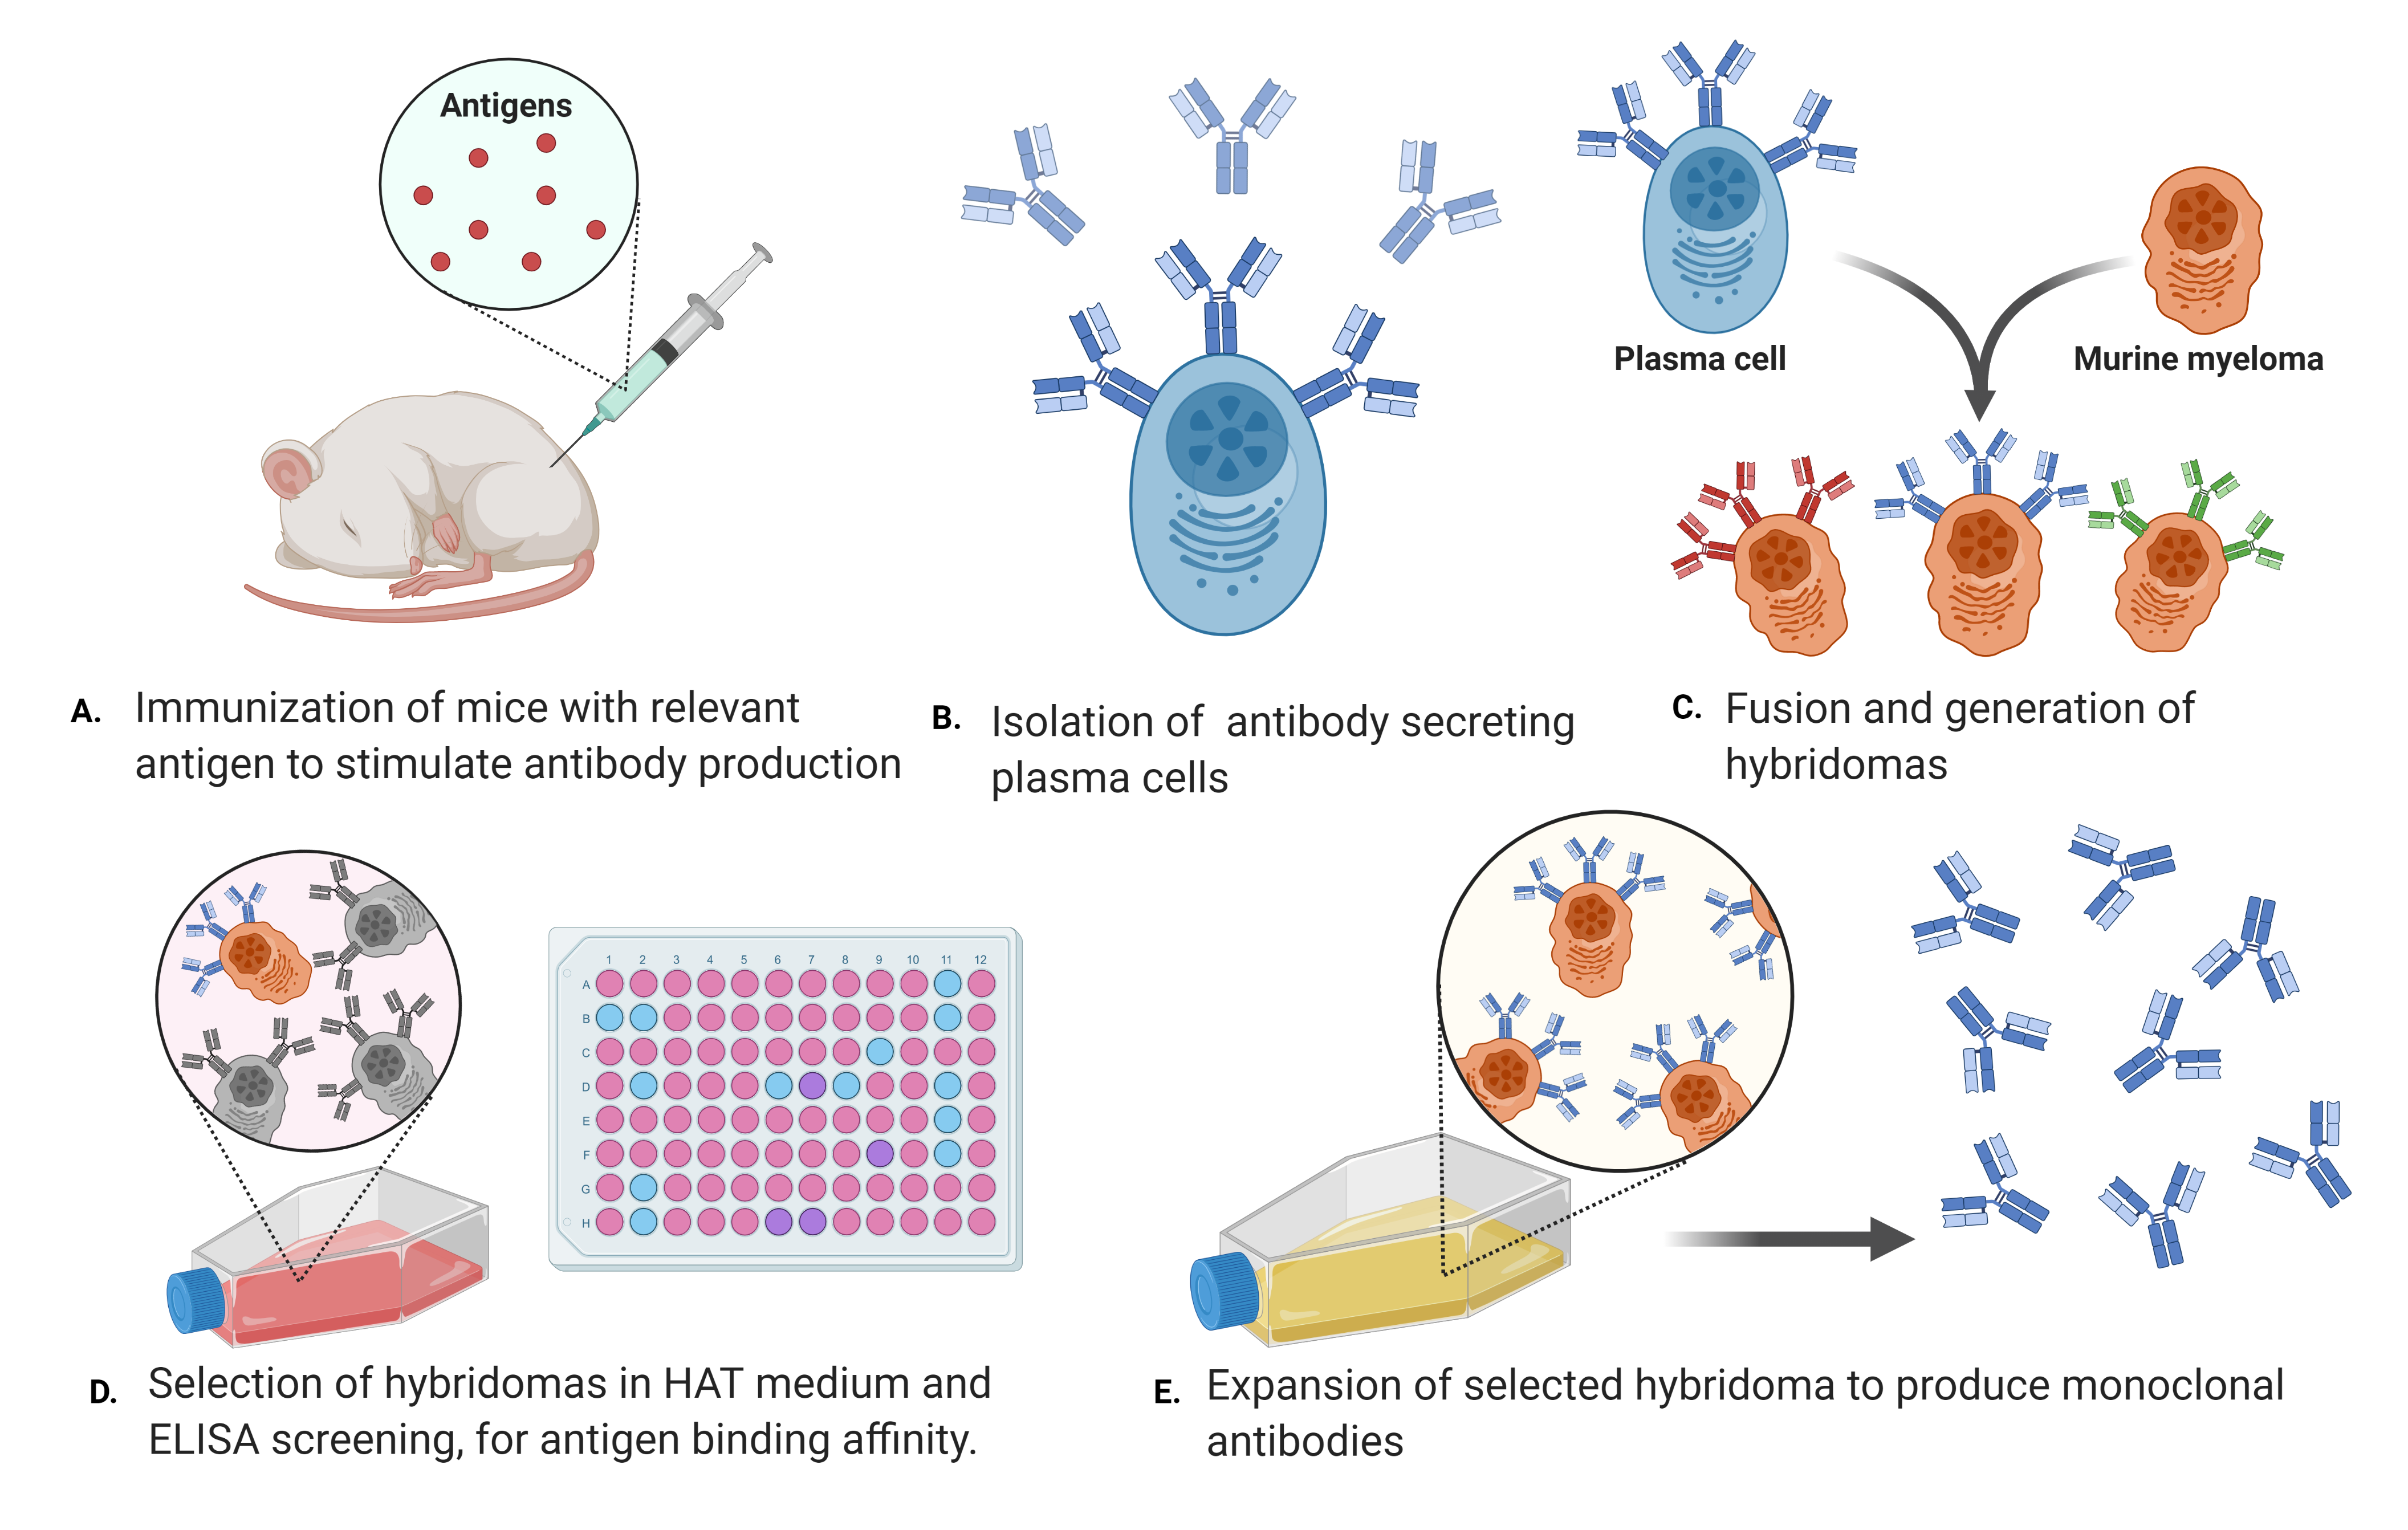
\includegraphics[width=0.9\linewidth]{./images/mabsproduction.png}
    \caption{\textbf{Production of murine mAbs via hybridoma formation. Author adapted from “Monoclonal Antibodies Production”, by BioRender.com} A. Antigens are injected into the mouse stimulating plasma cell formation. B \& C. Antibodies are isolated and fused with hybridomas. D. Hybridomas undergo selection pressure via the HAT medium to remove myeloma cells. E. Expansion to produce many monoclonal antibodies. } 
    \label{fig:mabsproduction}
\end{figure}

\subsection{Human Monoclonal Antibodies}

Fully human monoclonal antibodies can be produced via hybridoma techniques with transgenic mice \cite{lonbergAntigenspecificHumanAntibodies1994}. A faster but more expensive alternative to the hybridoma technique produces recombinant monoclonal antibodies (rAbs). The method was introduced by S.F.Parmley and G.P.Smith after Smith demonstrated a phage could present polypeptides on its surface \cite{parmleyAntibodyselectableFilamentousFd1988,smithFilamentousFusionPhage1985}. This technique, denominated phage display, requires a library of phage viruses. Initially, mRNA must be extracted from human B lymphocytes, which is used to create complementary DNA (cDNA) via a reverse transcription polymerase chain reaction (PCR) method. A set of primers designed to bind DNA responsible for the heavy and light chain regions of the antibody are used in PCR. Once amplified these cDNA copies are randomly joined and inserted into suitable phagemids via restriction enzymes and linker DNA, M13 phagemids are commonly used due to their mechanism of chronic infection, yielding a high output of reproduced phages from the bacteria. The recombinant phagemids are then inserted into \emph{E.Coli} along with the rest of the phage genome from a helper phage. The \emph{E.Coli} produce phages with single-chain fragment variable (scFvs) or F\textsubscript{ab} regions (\textbf{Figure \ref{fig:AntibodyStructure}}) present on their cell surface. Once a library is established, an antigen can be presented, phages that bind with a high affinity to the antigen will remain in the library while weakly binding phages are washed away. This is repeated to find high-affinity mAbs, and is known as bio-panning (\textbf{Figure \ref{fig:phagepanning}}) \cite{azzazyPhageDisplayTechnology2002, marksBypassingImmunization1991}. Once phages with high binding affinity have been separated they can be sequenced and analysed to find common and conserved residues via computational methods. Whilst phage display is a faster method, it is more expensive and resulting antibodies often have less affinity for their antigen.

\begin{figure}[h!]
    \centering
    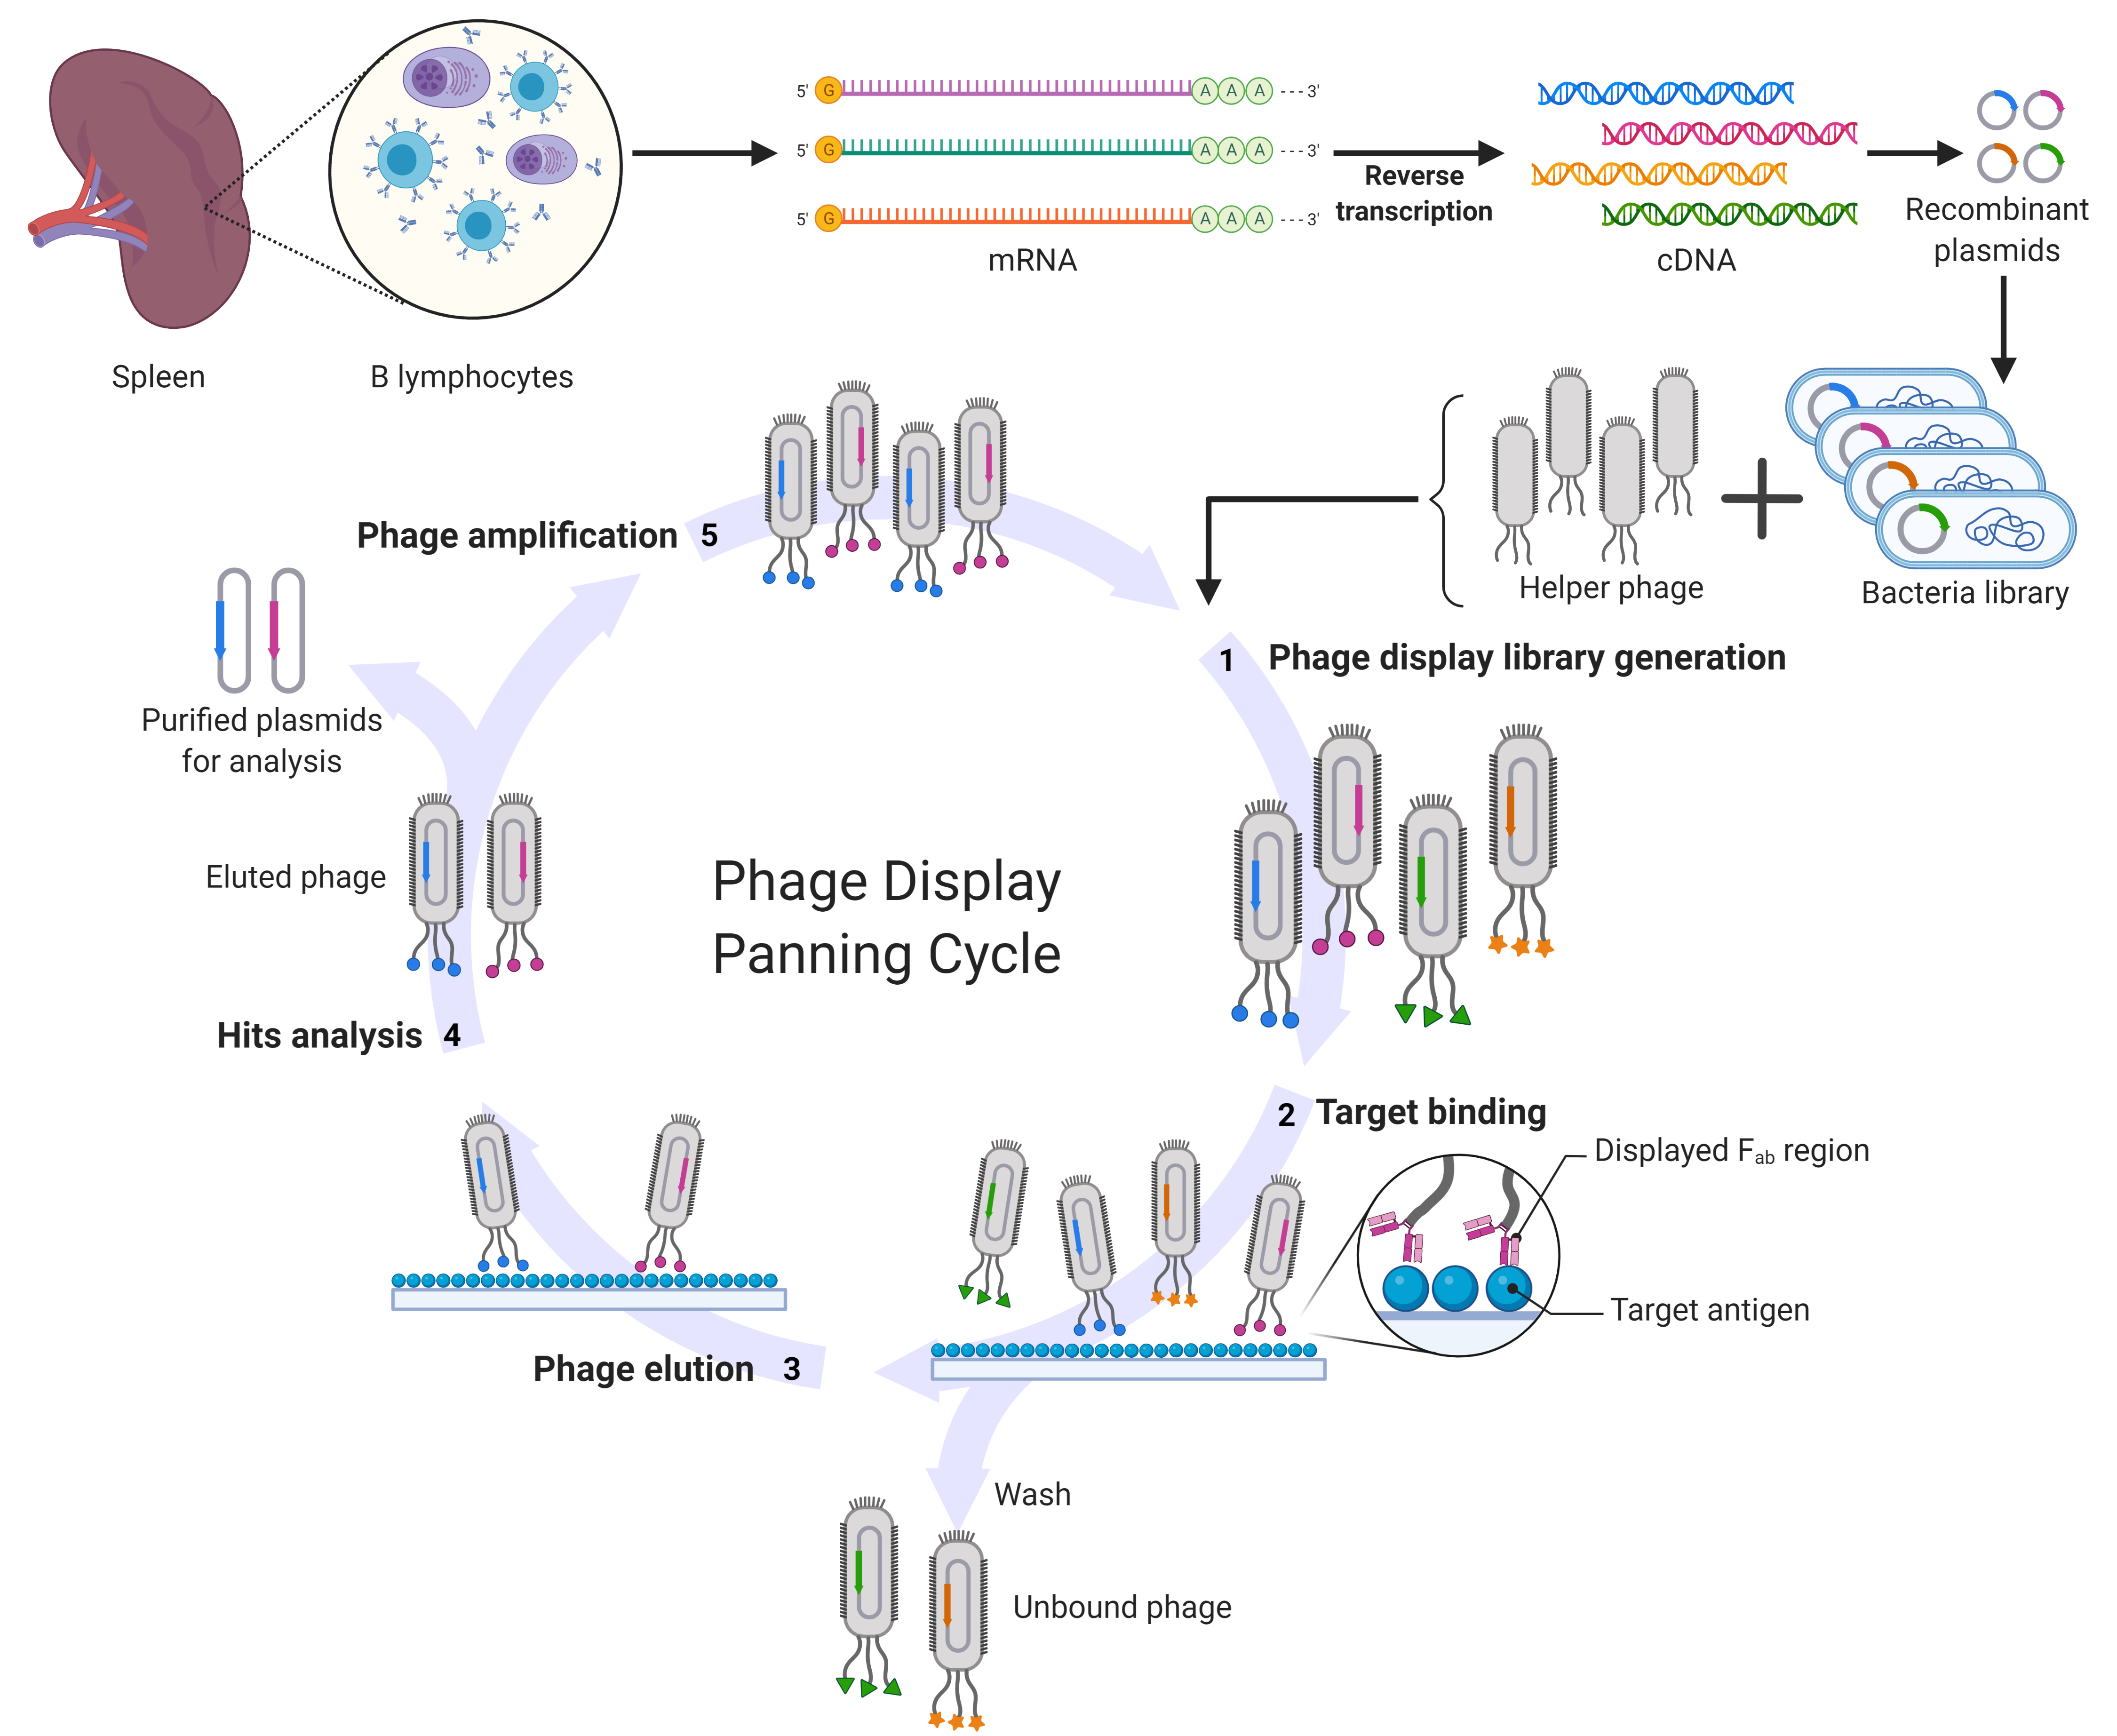
\includegraphics[width=1\linewidth]{./images/phagepanning.png}
    \caption{\textbf{Phage panning as part of the phage display method. Author adapted from “Phage Display Panning”, by BioRender.com}
    mRNA extracted from B lymphocytes in the donor's spleen undergoes reverse transcription to cDNA where PCR amplifies specific antibody associated DNA. DNA is then inserted into a plasmid vector and expressed in \emph{E.Coli}. After formation of the phage library, target binding of antibody occurs and unbound phages are washed away. The phagemids are then extracted from eluted phage and sequenced.} 
    \label{fig:phagepanning}
\end{figure}

\subsection{Current therapeutics and diagnostics}

Some major examples of mAbs as therapeutics are adalimumab, rituximab, and bevacizumab. Adalimumab, a human rAb, treats various types of arthritis by targeting tumour necrosis factor, a substance associated with severe forms of arthritic diseases \cite{measeAdalimumabTreatmentArthritis2007}. Bevacizumab, a humanised mAb cancer treatment, targets circulating VEGF which promotes rapid proliferation in cells, thus binding to this will prevent signaling via the VEGF receptor and cause a reduction in cell proliferation \cite{kazazi-hyseniBevacizumab2010}. Rituximab, a chimeric antibody, targets the CD20 ligand on B lymphocytes in immune-related diseases such as autoimmunity, resulting in a depletion of these lymphocytes \cite{thurlingsSynovialTissueResponse2008}, trials of patients with Pemphigus vulgaris showed that B lymphocyte population dropped within 20 hours of treatment and remained low for 12 months \cite{emingRituximabExertsDual2008}. Whilst there is a sizeable market for these mAbs there are many downsides: they are incredibly expensive and time-consuming to produce, there are ethical considerations in producing hybridomas, and paratopes can be non-specific leading to undesired side effects \cite{saylorMonoclonalAntibodybasedTherapies2009}.

\subsection{The need for computational power}

As explained, the processes to produce mAbs is currently very long winded, expensive and can result in antibodies with weak affinity for the target antigen. Antigens are any molecules that elicit an immune response and therefore can be virtually any substance; usually, they are proteins, peptides, or polysaccharides that form parts of the exterior of pathogens. Due to the specificity of mature antibodies, a hugely diverse range of binding regions are necessary to bind as many antigens as possible, this is achieved through a specialised splicing process named somatic recombination. The variable region of the light chain (V\textsubscript{L}) is encoded by two DNA segments: the variable and joining gene segments which contain many similar domains. Additionally, the heavy chain has an extra domain named the diversity gene segment; these separate exons are rearranged or spliced and joined via RNA splicing (\textbf{Figure \ref{fig:SomaticRecombination}}) \cite{rothRecombinationMechanismErrors2014}. Due to this random rearrangement and selection within each segment, it is thought that there could be as many as 10\textsuperscript{11} unique antibody molecules in a single individual \cite{glanvillePreciseDeterminationDiversity2009}. 
\\[12pt]
Computers perform billions of operations every second, and therefore the ability to model a 3D epitope structure, find an antibody with a complementary binding site and determine the sequence of said resulting structure would lead to faster and cheaper design of higher quality mAbs. This would be incredibly advantageous in designing antibodies. According to the Structural Antibody Database \cite{dunbarSAbDabStructuralAntibody2014} only 3500 antibody structures are present in the Protein Data Bank (PDB) \cite{bermanProteinDataBank2000a}, the main source of protein 3D structures. Traditional techniques such as nuclear magnetic resonance (NMR) and X-ray crystallography are laborious and expensive tasks, therefore a computational based approach could save time and money ensuring lab experiments are targeted at structures with potential, or even solve protein 3D structures from the genetic sequence to avoid hybridoma or phage display techniques altogether.

\begin{figure}
    \centering
    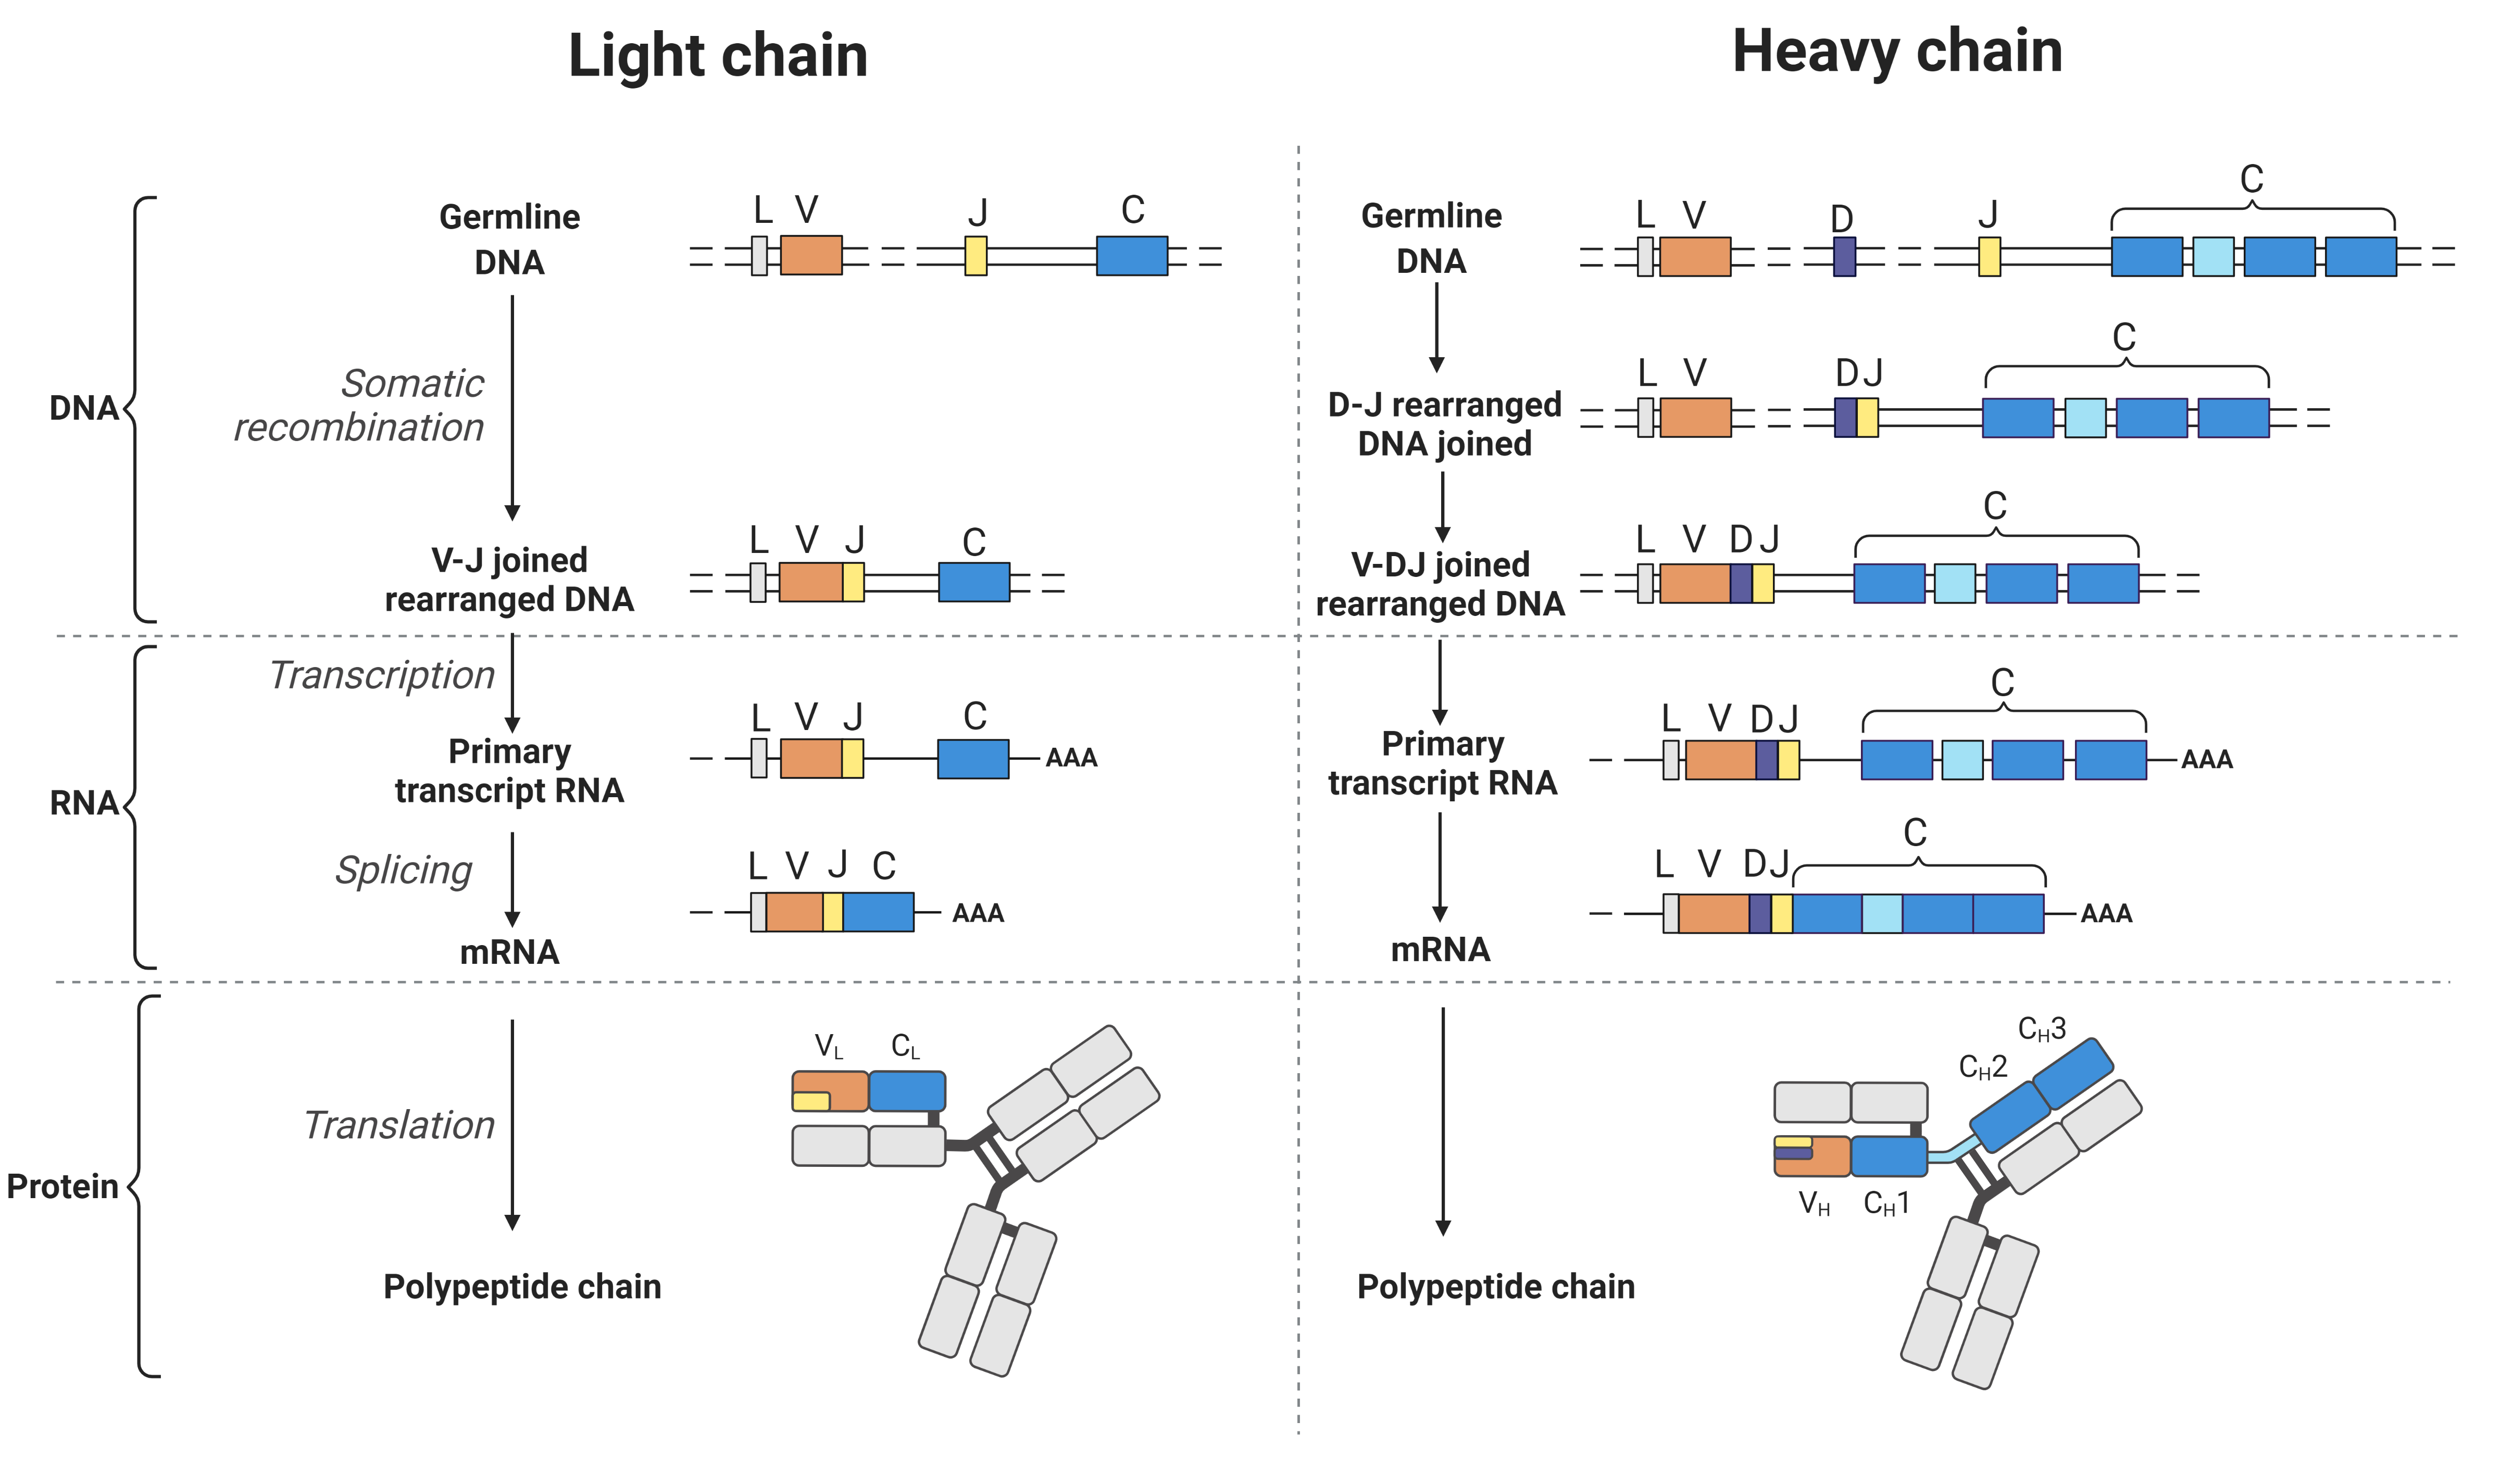
\includegraphics[width=\linewidth]{./images/somaticrecombination.png}
    \caption{\textbf{Somatic recombination in heavy and light variable regions} increases the variety of paratopes for antigen binding. Variable (V) and Joining (J) segments provide variety within the V\textsubscript{L} chain, whereas the V\textsubscript{H} chain has an additional diversity segment. These segments help form the variable paratopes of immunoglobulin proteins. Made with biorender.com}
    \label{fig:SomaticRecombination}
\end{figure}



\subsection{Introduction to deep learning}

Machine learning is the study of computer algorithms that can improve themselves using data without human intervention. Deep learning is a subset of machine learning and applies many algorithms in layers to form a neural network (NN), like that of the human brain \cite{estevaGuideDeepLearning2019}. 

\textbf{\subsubsection{Convolutional Neural Networks}}

Convolutional Neural Networks (CNNs) are incredibly popular and have existed for quite some time, they are normally applied to image classification \cite{krizhevskyImageNetClassificationDeep2017} and object recognition \cite{zhangImprovingObjectDetection2015}. A CNN maintains the basic structure of a neural network with layers of interconnected artificial neurons; but applies filters to the inputs of the NN. A filter is just a mathematical operation applied to every input in the input layer, the filter slides over each square to produce a feature map. When applied to images, early feature maps are often basic segments of objects such as edges or patches of colour. These feature maps are enriched with more convolutional layers, and more training iterations; which form more complex features describing the image, these are called high-level feature maps and can be used to classify objects in images. It is reasonable to assume that increasing the number of layers, leads to richer feature maps which lead to better object identification, which is true to an extent. More layers create higher-level features, but there is point at which the model becomes too deep and complex and proceeds to perform poorly (\textbf{Figure \ref{fig:resnet_compare}})\cite{heDeepResidualLearning2016}. This poor performance is due to a problem known as the vanishing gradient problem \cite{bengioLearningLongtermDependencies1994}, this relates to the mathematical function that neurons within the neural network apply to the inputs, if the inputs are too large, the gradient that updates the NN parameters can become diminishingly smaller until it has little to no effect. To solve this problem a new architecture was introduced, that forms residual neural networks (ResNets) \cite{heDeepResidualLearning2016}.

\begin{figure}[h!]
    \centering
    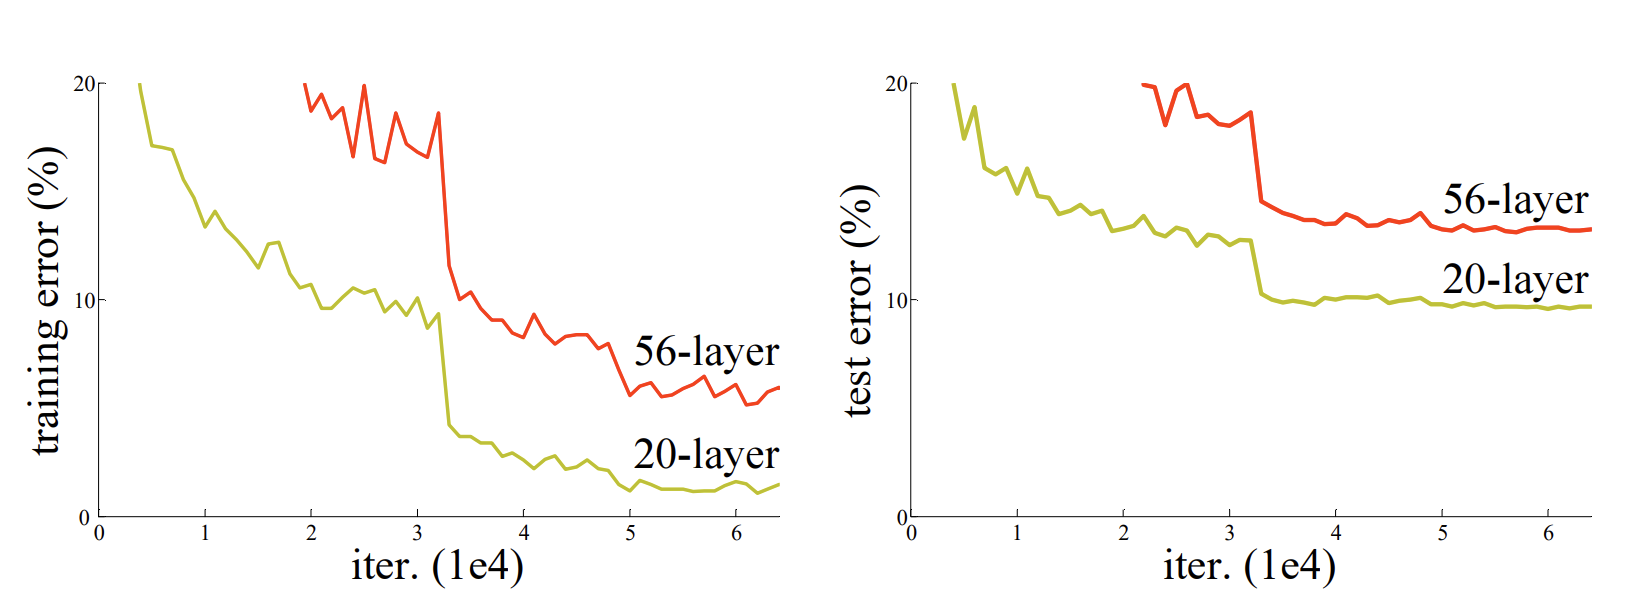
\includegraphics[width=0.95\linewidth]{./images/graph_resent_cnn.png}
    \caption{\textbf{Training and test error of a 20 and 56 layer CNN.} training (left) and test (right) error vs iterations. Red line shows a deep CNN and the green a shallower CNN. Image sourced from (he et al. Deep Residual Learning for Image Recognition. 2016) \cite{heDeepResidualLearning2016} }
    \label{fig:resnet_compare}
\end{figure}

\textbf{\subsubsection{Residual Neural Networks}}

Residual neural networks (ResNets) are a sub-category of CNN which also utilise filters to automatically extract features from the provided data set during training. ResNets differ from CNNs in the structure of their networks; additional to the fully interconnected neural network there are skip connections. Skip connections connect the input of a neuron to its output, essentially allowing a neuron to be bypassed. This ensures two things: Firstly, each network layer will perform at least as well as it did on previous iterations as the data can skip this layer and remain unmodified, and this will occur naturally by chance on certain repetitions of training. If the unmodified data is the optimal output then it is selected thus preventing an irregular neuron or layer affecting output \cite{heDeepResidualLearning2016}. Furthermore, on each iteration of training, there is a backpropagation state, in which the parameters for each neuron are adjusted based on the difference between the output of the network data and the labelled training data. The option to travel through a skip connection on the backpropagation stage allows the gradient to jump back to previous neurons thus preventing the reduction of its value in every layer \cite{heDeepResidualLearning2016}. This allows ResNets to be trained to a much deeper level than CNNs (\textbf{Figure \ref{fig:resnet_performance}}), making them more accurate in labelling real world data with extracted features.


\begin{figure}[h!]
    \centering
    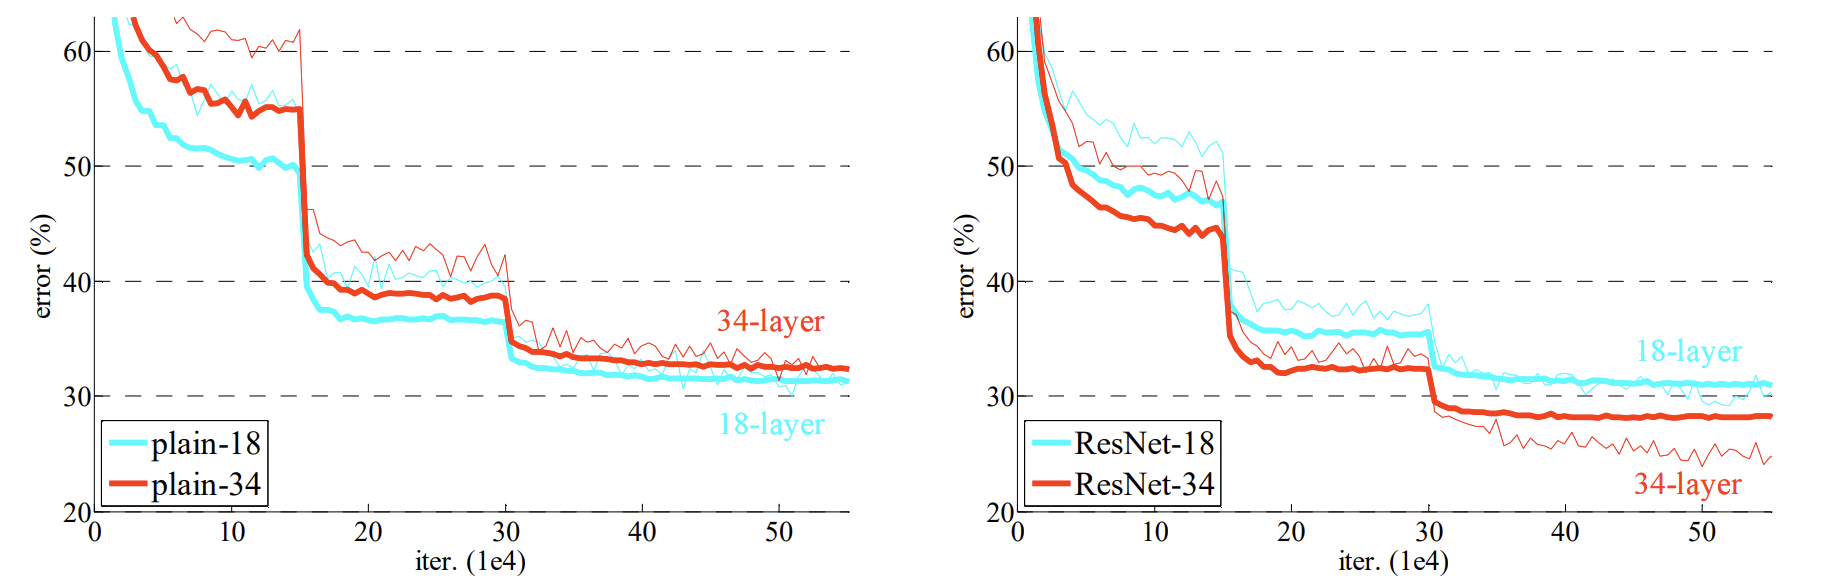
\includegraphics[width=0.95\linewidth]{./images/resnet_performance.png}
    \caption{\textbf{Comparison of basic CNN (left) and ResNet (right) at different depths}. Plain CNN and ResNets had the same number of parameters to ensure fairness in comparison. Image sourced from (he et al. Deep Residual Learning for Image Recognition. 2016) \cite{heDeepResidualLearning2016}}
    \label{fig:resnet_performance}
\end{figure}

\textbf{\subsubsection{Recurrent and Long Short-Term Memory Neural networks}}

Recurrent neural networks (RNNs) \cite{bengioLearningLongtermDependencies1994} are iterative, thus a layers output loops back into the input as to consistently extract more features, they are commonly used in tasks such as speech recognition and translation. RNNs are more complex than conventional NNs, they posses an internal state, that can memorise information about previous inputs. Unfortunately, the promise of memory falls flat in practise as RNNs fail to learn over large numbers of iterations, as older inputs present in the state become vanishingly small. To tackle this problem, long short-term memory neural networks (LSTMs) were introduced \cite{gravesFramewisePhonemeClassification2005}. LSTMs are a special kind of RNN that can learn and remember data over long periods of time. They achieve this by replacing the single repeating structure of a RNN with 4 channels, which each represent a different state. Layers range from no memory to only long term memory, and thus with numerous iterations, channels are selected by chance and different states of memory are expressed within the NN \cite{hochreiterLongShortTermMemory1997}. This recollection of data proves very useful in some scenarios.

\textbf{\subsubsection{Point Neural Networks}}

Point Neural Networks (PointNets) \cite{qiPointNetDeepLearning2017} are optimised to interpret point cloud data. Point cloud refers to data that represents points in space, that contribute to a 3D structure. Unlike images which is a grid of pixels, 3D data is unstructured and therefore harder to convert  into an input recognisable to a computer. PointNets utilise a spatial transformer network \cite{jaderbergSpatialTransformerNetworks2016}, which maintains the input's geometric features whilst applying filters similar to those in the CNN, this allows automatic feature extraction for 3D objects.


\textbf{\subsubsection{Difficulties}}

A drawback to deep learning is the quantity of data the algorithms require to apply weights to their models and ‘learn’. Although the boom in popularity of deep learning over the last few years is partly due to the recent developments in genome sequencing, resulting in a large amount of accessible genomic data in the public domain. Another concern around more complex NNs such as CNNs, ResNets, and PointNets is overfitting.
There can be multiple factors that play into overfitting but usually a complex model is trained on an insufficient volume of data, the result is a model that memorises the training data and specifically tailors its output to the training data set and thus will not perform well with real world data. There are a few different methods utilised in countering overfitting: Data augmentation, disturb label, weight decay, and dropout are a few of examples.
\\[12pt]
Data augmentation can diversify a training data set without the need for any additional data. The technique involves manipulating the existing data to produce slight variations of the same input, for example in image processing, rotating or cropping the images. This diversification essentially provides more training data for the NN to train from, reducing the likeliness of an overfit \cite{mikolajczykDataAugmentationImproving2018}.
\\[12pt]
DisturbLabel \cite{xieDisturbLabelRegularizingCNN2016} and dropout \cite{srivastavaDropoutSimpleWay2014a} are executed in a similar manner. DisturbLabel acts after each training iteration as the parameters are being updated in the neural network, by introducing random noise, and preventing the neural network from relying on specific bloated parameters. Dropout, affects neurons in the forward training route, and in the backwards readjustment phase, by randomly ignoring some neurons within each iteration, again preventing the reliance on small numbers of neurons for big changes in output. These both promote more robust features to remain in the feature maps, and reduces the chance of noise and other smaller connections being prioritised \cite{xieDisturbLabelRegularizingCNN2016, srivastavaDropoutSimpleWay2014a}.
\\[12pt]
Weight decay is a fairly simple method of reducing overfitting, and acts during the training phase on certain parameters that are being applied to the inputs of the hidden layers within a neural network. This technique penalises parameters that become to large, preventing a small group of parameters from dominating the output of the network \cite{kroghSimpleWeightDecay1991}. 
\\[12pt]
All of these overfitting prevention techniques result in more iterations required during the training stage, meaning more time spent training and higher server costs, but ensure only relevant features are being added to the feature map. 

\textbf{\subsubsection{Implementations}}

The research in this dissertation was partly inspired by a program named AlphaFold \cite{seniorImprovedProteinStructure2020}, it highlights the potential of deep learning techniques.
\\[24pt]
AlphaFold is a cutting-edge deep learning technology that predicts tertiary protein structure from its genetic sequence. The software was entered into the Critical Assessment of Protein Structure Prediction or CASP13 (2018) along with 97 other teams; Teams are ranked on many criteria across many protein predictions, but the main metric is known as the global distance test (GDT), which scores from 0-100, and counts the percentage of atoms within a threshold distance of the experimentally calculated protein structure. During the 2018 CASP13 assessment the AlphaFold team scored just under 60 in the GDT test average \cite{seniorImprovedProteinStructure2020} and was recognised as the best software entered into the competition. Wanting to improve, the team resubmitted a completely re-engineered version: AlphaFold2 in CASP14 2020 and score a median of 92.4 across all targets, with their predictions having an average error (RMSD) of approximately 1.6 Angstroms \cite{jumperHighAccuracyProtein2021}.
\\[24pt]
Similar methods of deep learning could be applied in many ways to aid in the design of antibodies. Structural predictions can be made about the antibody and its paratope, using template models from the PDB or \emph{ab initio} modelling \cite{choongComputerAidedAntibodyDesign2017} from just a peptide sequence. Structural predictions can also be made about the epitope on the surface of the antigen. From these structures, a docking simulation can be performed to calculate the binding affinity between antibody and antigen; then through a feedback loop with refinement this tool could accurately assign a highly specific protein structure for a provided antigen \cite{kringelumReliableCellEpitope2012}.

\section{About this dissertation}

This dissertation aims to answer the question: "How effective is Deep Learning in therapeutic antibody development?". I will break the research into two distinct segments: 3D paratope and epitope structure prediction and paratope-antigen docking simulations. I will evaluate the varying methodologies throughout some selected literature to investigate which techniques and architectures are most effective at predicting antibody and antigen structure and their interactions. Additionally, I will highlight the limitations of certain techniques and explain how these papers can be applied in real world scenarios.
